%% Graphical Abstract Text (J-BHI). Standalone one-page PDF for the separate upload slot.
\documentclass[11pt,a4paper]{article}
\usepackage[T1]{fontenc}\usepackage[utf8]{inputenc}\usepackage{lmodern}\usepackage{microtype}
\usepackage[margin=2.4cm]{geometry}\usepackage{graphicx}\usepackage[hidelinks]{hyperref}
\setlength{\parskip}{0.5em}\setlength{\parindent}{0pt}
\begin{document}
\begin{center}
{\large\bfseries Graphical Abstract Text}\\[1.0em]
{\Large\bfseries Subject-Wise Evaluation Exposing Identity Leakage in Actigraphy-Based Mental-Health Prediction}\\[0.6em]
{\normalsize Aminat Abiola Ajibola, University of Hafr Al-Batin}\\[1.2em]
\end{center}
\textbf{Table-of-contents caption (50 words).} Actigraphy models for depression, schizophrenia and ADHD lose 0.04 to 0.15 AUROC when evaluated subject-wise instead of day-wise. Day-wise models score above chance on shuffled labels and re-identify participants from one day at 27 to 40 percent, showing they learn identity; published accuracies above the honest band used day-level splits.

\vspace{1.2em}\textbf{Accompanying image} (uploaded separately as \texttt{graphical\_abstract.png}, 3900\,$\times$\,1980 px, 300 dpi):

\vspace{0.6em}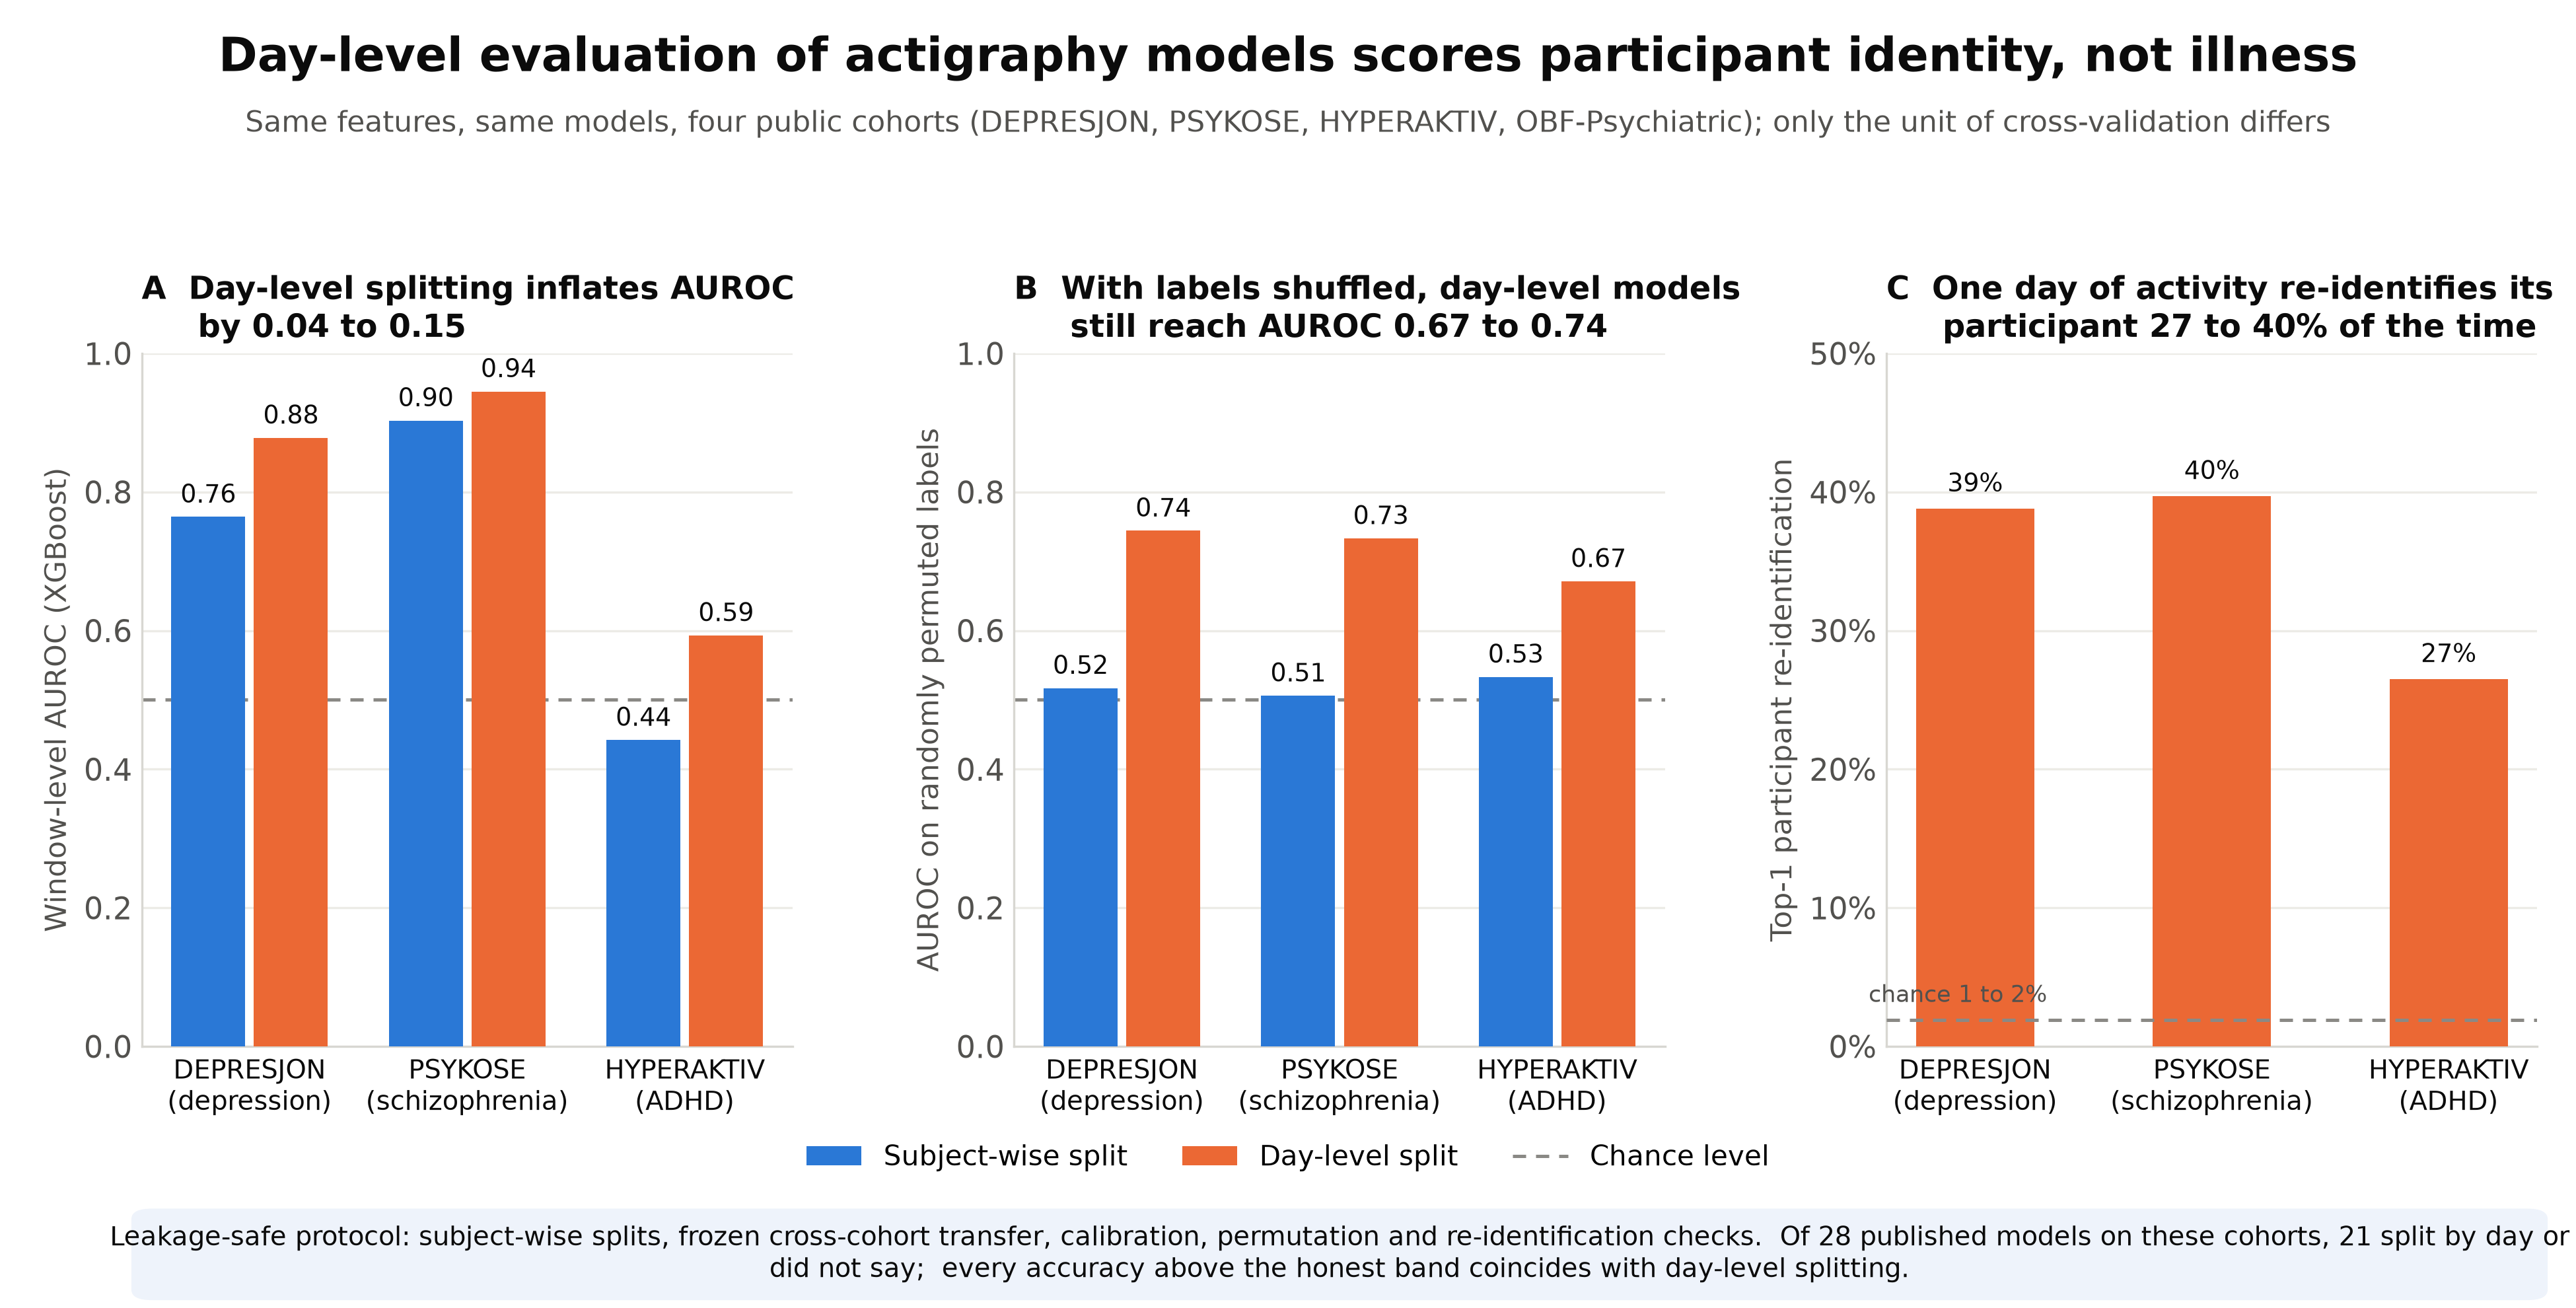
\includegraphics[width=\linewidth]{graphical_abstract.png}
\end{document}
